% ---------------------------------------------
% LaTeX Arquivo para Currículos
% Adicione na mesma pasta o arquivo: res.cls
% ---------------------------------------------
\documentclass{res}

\usepackage[english]{babel}
\usepackage[utf8x]{inputenc}
\usepackage{fancyhdr}  % manter 2 linhas no cabeçalho
\usepackage{graphicx}  % adicionar imagens
\usepackage{url}       % adicionar páginas

\renewcommand{\headrulewidth}{0pt} % suprime a linha do cabeçalho
\setlength{\headsep}{24pt}  % espaço entre o cabeçalho e o texto
\setlength{\headheight}{24pt} % permite a 2a. linha do cabeçalho
\pagestyle{fancy} % estilo da pagina
\rhead{ {\it F. Anselmo}\\{\it pág. \thepage} } % cabeçalho da 2a. página
\cfoot{} % rodape vazio
\topmargin=-0.5in % start text higher on the page

\begin{document}
	
	\thispagestyle{empty} % Esta página não possui cabeçalho
	\name{FERNANDO ANSELMO\\[5pt]}
	\address{{\bf Brasil - DF - Brasília} -- Asa Norte -- 70757-120 \\
		Tel. (61) 99874.0763 -- Tel.Recado (61) 3201.5834 \\
	    fernando.anselmo74@gmail.com}
	
	\begin{resume}
		
		\section{RESUMO PROFISSIONAL}
		\vspace{8pt}
		Fortes conhecimentos em linguagens de programação Java e Python. Especialista formado em Gestão da Tecnologia da Informação com forte experiência em Bancos Relacionais e não Relacionais. Possui habilidades analíticas necessárias para encontrar a providencial agulha no palheiro dos dados recolhidos pela empresa. Responsável pelo desenvolvimento de dashboards com a capacidade para analise de dados e detectar tendências, autor de 16 livros e diversos artigos em revistas especializadas, palestrante em seminários sobre tecnologia. Focado em aprender e trazer mudanças para a organização com conhecimento profundo do negócio.
		
		\section{HABILIDADES}
		\vspace{8pt}
		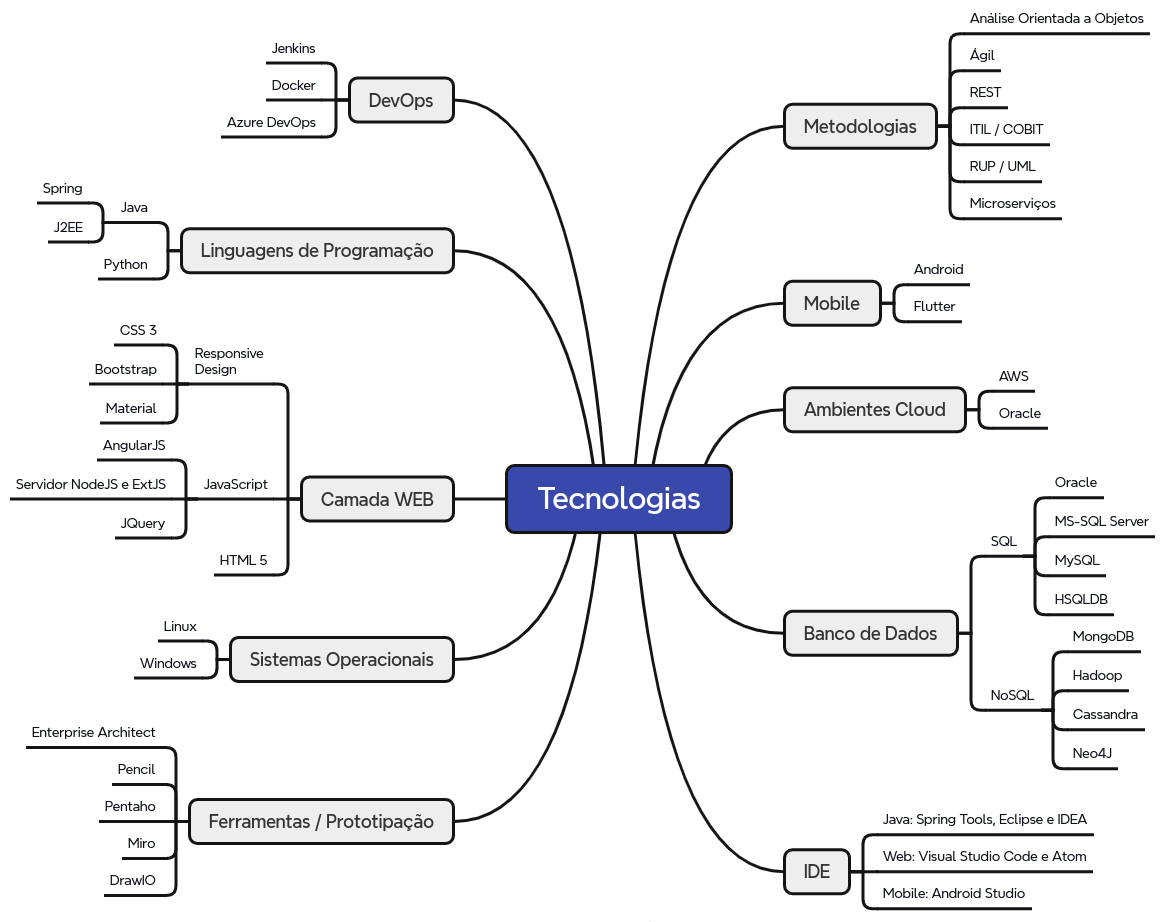
\includegraphics[width=0.9\textwidth]{imagens/tecnologias.png}
		
		\section{CERTIFICAÇÕES E TÍTULOS}
		\vspace{8pt}
		{\sl Ciências de Dados}, Formação Completa dos Cursos da Cognitive Class \hfill Jan/2019 \\
		{\sl SCRUM Foundation}, Diversas Empresas Certificadoras \hfill Jun/2019 \\
		{\sl Java Champion}, Oracle \hfill Dez/2006 \\
		{\sl Sun Certified Programmer for the Java 2 Platform 1.4}, Sun Microsystems \hfill Mai/2004 \\
		{\sl Java Standard Edition 6 Programmer Certified Professional}, Oracle \hfill Jan/2013 \\
		{\sl Java Enterprise Edition 5 Web Component Developer Certified Professional}, Oracle \hfill Jan/2013 \\
		{\sl Oracle 10g Database Specialist Sales Champion}, Oracle \hfill Jan/2008 \\
		{\sl Oracle 10g Technical Presales Champion}, Oracle \hfill Jan/2008 \\
		{\sl Diversos certificados em cursos oficiais SAP, Microsoft, Oracle, Unisys e RCM}
		
		\section{IDIOMAS} 
		\vspace{18pt}
		\begin{description}
			\item[Inglês] -- Nível avançado tanto para leitura como para escrita.
			\item[Espanhol] -- Nível avançado tanto para leitura como para escrita.
		\end{description}
		
		\section{EDUCAÇÃO}
		\vspace{8pt} 
		{\sl Especialização}: Faculdades Integradas da Católica | Programação de Computadores 
		\hfill Dez/1996 \\
		{\sl Graduação}: Universidade FacSenac | Gestão da Tecnologia da Informação     
		\hfill Dez/2011 \\
		{\sl Pós-Graduação}: Faculdade JK | Em Gestão Empresarial Avançada 
		\hfill Fev/2016 \\
		{\sl Técnico em Programação}: Instituto Federal de Educação, Ciência e Tecnologia de Brasília | Em Jogos Digitais
		\hfill Jan/2019 \\
		{\sl Pós-Graduação}: Faculdade Anhaguera | Em Estatística Aplicada
		\hfill Jan/2020 \\
		
		\section{HISTÓRICO PROFISSIONAL} % Da mais nova para mais antiga
		\vspace{8pt}
		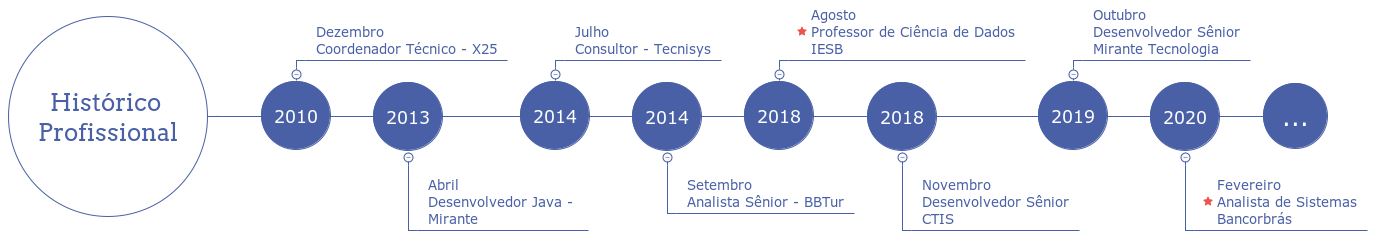
\includegraphics[width=1.0\textwidth]{imagens/experiencia.png}
		
		% Mais Recente
		{\sl Bancorbrás} \hfill Fev/2021 - Atual
		\begin{itemize}
			\item Devido aos excelentes serviços prestados, foi contratado pela Bancorbrás para compor o time de Arquitetura e definição de projetos Java com Spring Boot (Spring Data e Spring Batch), Jboss, Quarkus (GraalVM, Mensageria Assíncrona) e testes unitários (no padrão TDD). Montagem de ambiente de integração continua com: Docker, Jenkins 2, Sonar, Maven, Git. Com vivência em metodologias ágeis. Responsável por traduzir processos antigos em Stored Procedures da área de finanças para modernos em Linguagem Java e ambiente Spring Boot além de integrar aplicações Protheus e Active Directory para agilização dos processos de RH.
		\end{itemize}

		{\sl Mirante Tecnologia} \hfill Out/2019 - Fev/2021
		\begin{itemize}
			\item Contratado para prestar serviços de desenvolvimento de projetos de software para o cliente Bancorbrás. Utilização do framework Spring Boot para a construção de Micro Serviços para atender a empresa de modo Corporativo. Sincronização do ambiente com o uso do Jenkins/Docker para automatização e disponibilização de serviços. Desenvolvimento em tecnologia Java; Criação de testes unitários; Integração contínua e experiência na Cloud da Oracle. 
		\end{itemize}
		
		{\sl IESB} \hfill Ago/2018 - Atual
		\begin{itemize}
			\item Contratado como Professor na Pós e Graduação em Ciência de Dados. Com conhecimentos e habilidades para utilizar metodologias ativas na matéria de Introdução as Tecnologias de Ciência de Dados contemplando conhecimentos de Python, banco de dados Hadoop, Pensamento Analítico, Qualidade de Dados, Mineração de Dados e Big Data, Robótica e Automação.
		\end{itemize}
		
		{\sl CTIS} \hfill Nov/2018 - Out/2019
		\begin{itemize}
			\item Responsabilidades sob a absorção de novos sistemas, pelo seu andamento e preparação de documentos e ambientes para "Transferência de Tecnologia". Fornecimento de solução para problemas e definição das melhores práticas arquiteturais. Especificação técnica e desenho de arquitetura das soluções. Apoio e definição a estimativas técnicas das demandas. Acompanhamento de todo o ciclo de vida dos desenvolvimentos e realização as inspeções de código e auxílio aos desenvolvedores. Garantir que o produto em desenvolvimento está conforme a arquitetura definida. Apoio a equipe técnica nas dúvidas do dia-a-dia. Utilização de Ferramentas para gestão automatizada como o Nexus, Jenkins, Ansible e LiquidBase.
		\end{itemize}
		
		{\sl BB Turismo} \hfill Set/2014 - Nov/2018
		\begin{itemize}
			\item Atuou como como Analista de Sistemas Sênior e encarregado da manutenção e construção de projetos com tecnologia Java, JSF, JQuery, Hibernate em servidores JBoss e Base de dados SQL Server. Execução de um projeto Mobile com o uso de tecnologias PhoneGap, OnsenUI, Angular.js e JQuery. Responsável por organizar toda a comunicação de Voos e Hotéis com o WS/XML da Amadeus através de um servidor Ubuntu com Python para o envio e recebimento de REST/JSON.
		\end{itemize}
		
		{\sl Tecnisys Tecnologias Inovadoras} \hfill Jul/2014 - Ago/2014
		\begin{itemize}
			\item Atuou como Consultor em tecnologias Open Source. Instalação e configuração de projetos com o Jenkis e Nexus, além de ministrar treinamento com o JMeter para testadores.
		\end{itemize}
		
		{\sl Mirante Tecnologia} \hfill Abr/2013 - Jun/2014
		\begin{itemize}
			\item Alocado como Desenvolvedor Sênior Java para o cliente Cooperforte com o objetivo de realizar um projeto Ágil e uso metodologia Scrum. Projeto este que foi desenvolvido com a tecnologia JSF 2, JQuery, Hibernate em Servidores JBoss espelhados e utilização do Banco de Dados MS-SQL Server. Este projeto contou com o desenvolvimento realizado em várias camadas e seguiu os diversos padrões de projetos propostos, tais como, Façade, DAO, BO, VO, Factory Method entre outros. 
		\end{itemize}
		
		{\sl X25 Treinamento e Consultoria} \hfill   Dez/2010 - Mar/2013
		\begin{itemize}
			\item Levantamento e desenvolvimento de projetos internos no auxílio das atividades administrativas em linguagem Java, utilizando os frameworks Struts2, JSF e banco de dados PostgreSQL. Planejamento e desenvolvimento de treinamentos no modelo de Ensino à Distância. Seleção de uma base sólida de professores (baseado em experiência, certificações, hora-aula, didática, compromisso, entre outros). Instrutor dos cursos de Gerenciamento de Requisitos, Análise de Ponto de Função, Diversos na Carreira Java e Android. 
		\end{itemize}
		
		\section{EXPERIÊNCIA EM TRABALHOS VOLUNTÁRIOS E CAUSAS}
		\vspace{8pt} 
		{\sl DFJUG - Grupo de Usuários Java} -- Coordenador \hfill Jan/2000 - Nov/2016
		\begin{itemize}
			\item Moderador da lista, auxiliar nas atividades do projeto Rybená (\url{http://www.dfjug.org/rybena.jsp}) 
			que permite a comunicação via aparelhos móveis de deficientes auditivos. Responsável pela implementação 
			do Projeto JEDI no Brasil que visa o ensino de Java à Distância (\url{http://www.dfjug.org/jedi/index.jsp}).
		\end{itemize}
		
		{\sl Revista Segunda Empregável} -- Editor \hfill   Out/2013 - Out/2015
		\begin{itemize}
			\item Editor da revista semanal gratuita que auxilia os profissionais 
			que procuram uma colocação no mercado de trabalho (\url{http://fernandoanselmo.orgfree.com/wordpress/?page_id=173}).
		\end{itemize}
		
		\section{MAIORES INFORMAÇÕES}
		\vspace{18pt} 
		\begin{description}
			\item[Perfil no Linkedin] \url{http://www.linkedin.com/pub/fernando-anselmo/23/236/bb4}
			\item[GitHub] \url{https://github.com/fernandoans}
			\item[Canal no YouTube] \url{https://www.youtube.com/channel/UC4VS4Emzy0TSbfgMfWcpnxA}
			\item[Página Pessoal] \url{http://fernandoanselmo.orgfree.com/wordpress/}
			\item[Blog Pessoal] \url{http://fernandoanselmo.blogspot.com/}
		\end{description}
	\end{resume} 
\end{document}